%!TEX root = /Users/stevenmartell/Documents/CURRENT PROJECTS/iSCAM-trunk/fba/BC-herring-2011/WRITEUP/BCHerring2011.tex
\section{Results}
The results section is broken down into three major subsections, Maximum likelihood fits to the data, marginal posterior distributions, and stock forecasts and catch advice based on samples from the joint posterior distribution.

\subsection{Maximum likelihood fits to the data}
Although  the maximum likelihood estimates are not explicitly used for constructing the catch advice, we do present the MLE estimates of the residual patterns and fits to the data for comparisons.

\subsubsection{Catch residuals}
Residuals between the observed and predicted catch are largely determined by the user specified standard deviation in each of the control files.  In this assessment, the assumed variance for all regions (including minor regions) was set at 0.005, which corresponds to a standard deviation of approximately 0.0707.  Overall the residuals for each fishery in each stock assessment region are unremarkable (Fig. \ref{PartII:Results:fig1}), with exception of a  major outlier in the Haida Gwaii in the mide 1950s.  In 1956, the reported catch in Haida Gwaii was extremely large ($>$ 60,000 mt) and the model has a difficult time explaining this large catch. In order to explain this large catch in a single year, a large biomass in the region is required.

\begin{figure}[!tbp]
	% Requires \usepackage{graphicx}
	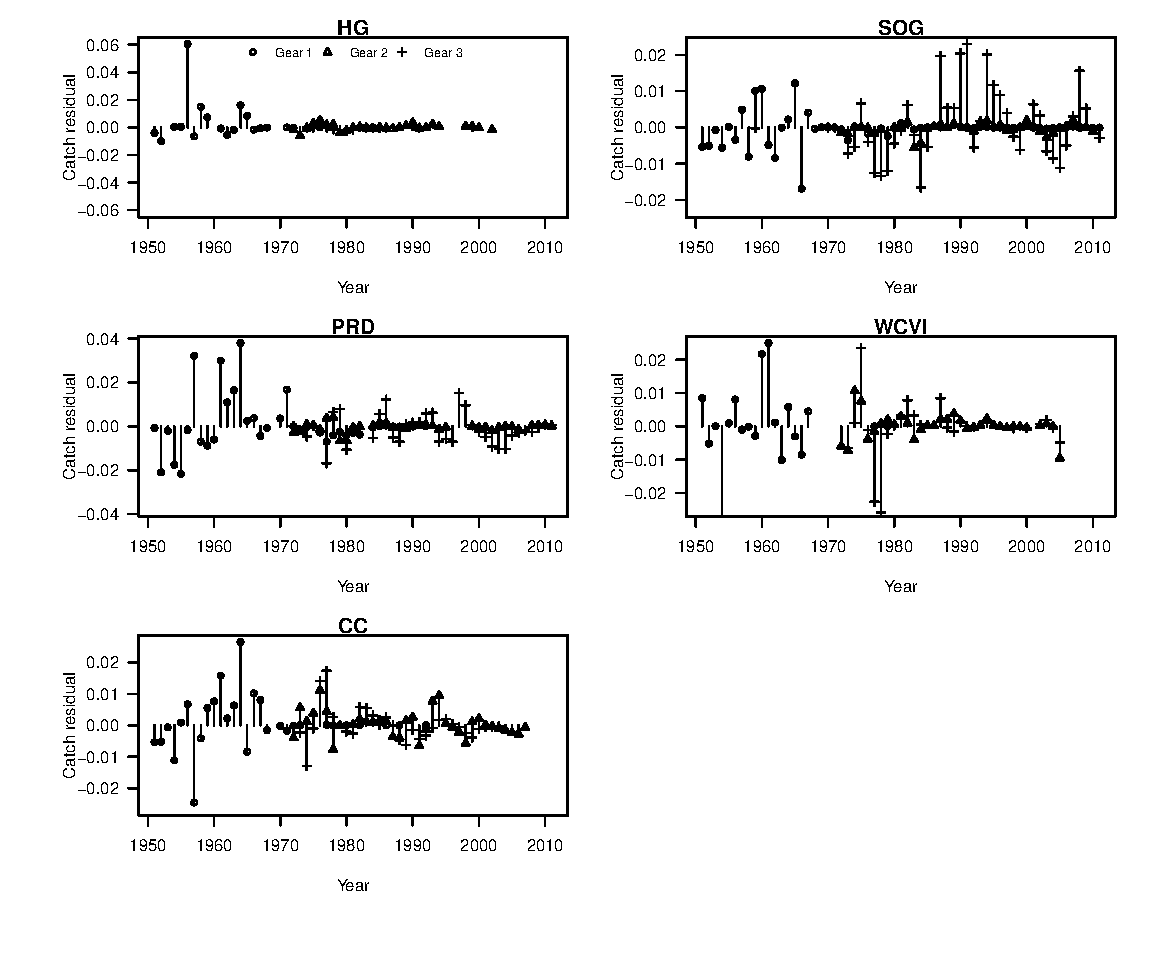
\includegraphics[width=\textwidth]{../FIGS/qPriorFigs/iscam_fig_catchresid.pdf}\\
	\caption{Residual for the log difference between observed and predicted catch for the five major SARs for each gear type (Gear 1 = winter seine fishery, Gear 2 = seine-roe fishery, Gear 3 = gill net fishery).}\label{PartII:Results:fig1}
\end{figure}


\subsubsection{Fits to the spawn survey data}
The residuals between the observed and predicted spawn survey index (on a log scale) are shown in Figure \ref{PartII:Results:fig2}.  Recall that the spawn survey data are treated as two independent time series where data between 1951--1987 were based on surface estimates of spawn area and data post 1988 are based on diver surveys of spawn area.  More weight was assigned to the contemporary data.   

For most areas, there is little pattern in the residuals between the observed and predicted survey data (Fig \ref{PartII:Results:fig2}).  For the HG, PRD and CC regions, there is very good correspondence between the observed and predicted survey data post 1988.  IN the SOG, there is a period of positive residuals between 1999 and 2005 where the predicted spawn biomass fails to increase as much as indicated by the survey.  Similary 3--4 year trends also exist in the WCVI spawn survey data after the year 2000.

\begin{figure}[!tbp]
	% Requires \usepackage{graphicx}
	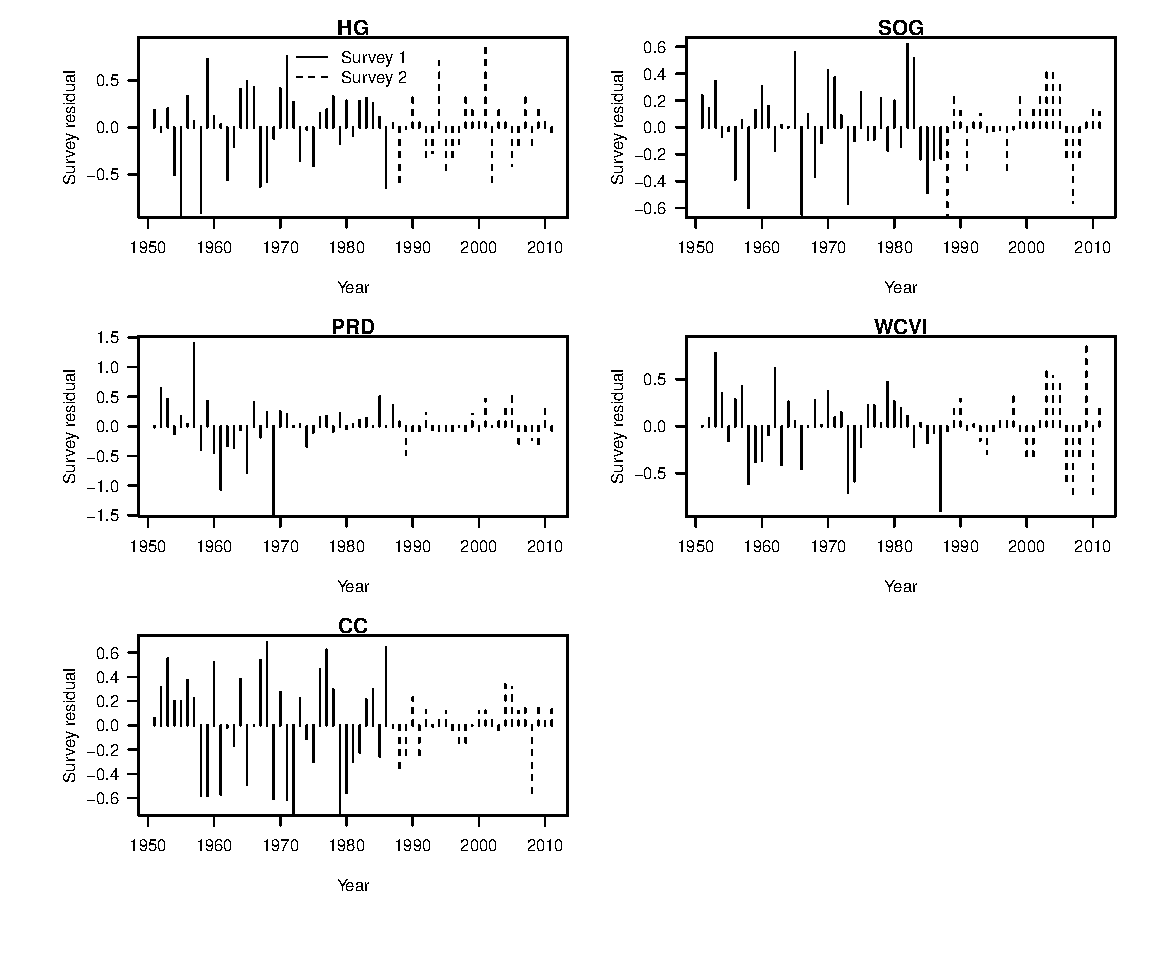
\includegraphics[width=\textwidth]{../FIGS/qPriorFigs/iscam_fig_surveyresid.pdf}\\
	\caption{Residual patterns for the log difference between observed and predicted spawn survey abundance for the five major SARs. Spawn survey data based on surface estimates are show as solid lines and data based on diver surveys is shown as dashed lines.}\label{PartII:Results:fig2}
\end{figure}

In comparison to the previous assessment for Pacific herring using the HCAM model, estimates of the catchability coefficient are very different (HCAM assumed q=1 for post 1988 data).  In each of the five major assessment regions (and the two minor regions) a less informative prior for the catchability coefficient was used (see Appendix \ref{Appendix::q_prior}).  Maximum Likelihood Estimates (MLE) of the catchability coefficients are presented for each region in Fig. \ref{PartII:Results:fig3} along with the observed and predicted trends in the spawn index.  Estimates of $q$ in both time periods are less than 1.0 for all regions with the exception of post 1988 data in the PRD region.  The interpretation of $q=1$ is that the spawn survey data is an absolute measure of spawn abundance, $q<1$ implies that the survey under-estimates the spawn abundance and $q>1$ implies an over-estimate.  For example, in the HG region the MLE values for $q$ are 0.245 and 0.433 for the pre- and post-1988 data, respectively. This could be interpreted as the spawn survey only, on average, sees 24.5\% and 43.3\% of the deposited spawn each year.  This interpretation however is conditional on the specification of mature biomass in the stock assessment model. 

\begin{figure}[!tbp]
	% Requires \usepackage{graphicx}
	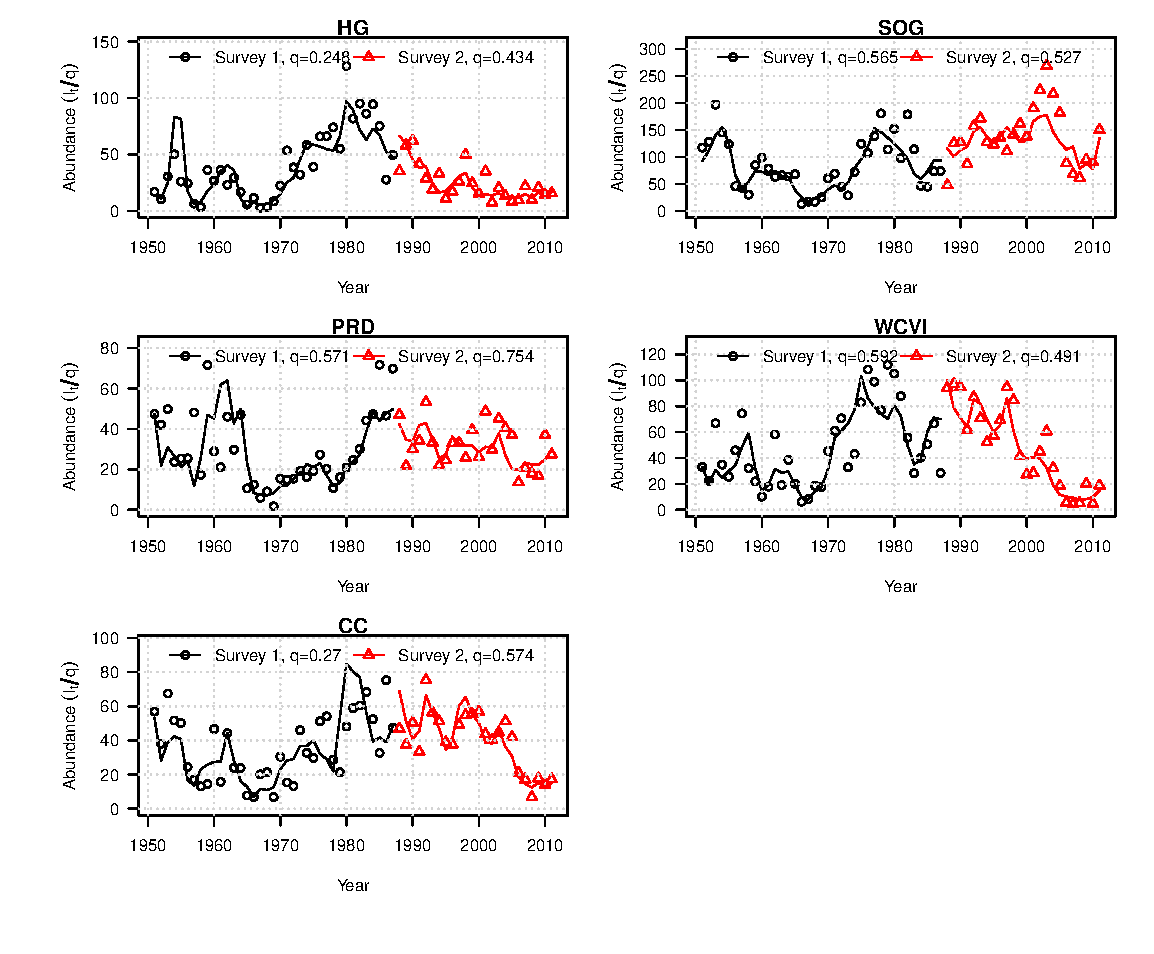
\includegraphics[width=\textwidth]{../FIGS/qPriorFigs/iscam_fig_surveyfit.pdf}\\
	\caption{Observed (points) and predicted (lines) relative abundance data (spawn survey data) for each of the five major SARs.  In each panel, the corresponding scaler ($q$) is presented for each of the surveys.}\label{PartII:Results:fig3}
\end{figure}


\subsubsection{Age composition residuals}

The assumed error distribution for the age-composition data has changed in this assessment from a multinomial distribution implemented in HCAM to a multivariate-logistic distribution. In the former implementation the age-composition data were weighted by the annual samples sizes in each region for each age and year. In the \iscam\ implementation the age-composition data for all years is given the same weight (i.e., we assume the observation errors is homogenous) based on the conditional maximum likelihood estimate of the variance (see Appendix \ref{appiSCAM} for full details).  We further pool age-proportions that are less than 2\% into the adjacent younger year class to reduce the influence of small outliers and weak cohorts.

In HG the MLE estimates of the variance for each gear is 0.102, 0.104 and 0.351, for the winter seine, seine-roe and gill net fleets, respectively (Fig. \ref{PartII:Results:figAgeCompHG}).  In general there is fairly good agreement between the observed and predicted age-composition data in this region, with poorer fits to the gill net age-composition data.  There is no persistent pattern in the residuals. 

\begin{sidewaysfigure}[!tbp]
	% Requires \usepackage{graphicx}
	\centering
	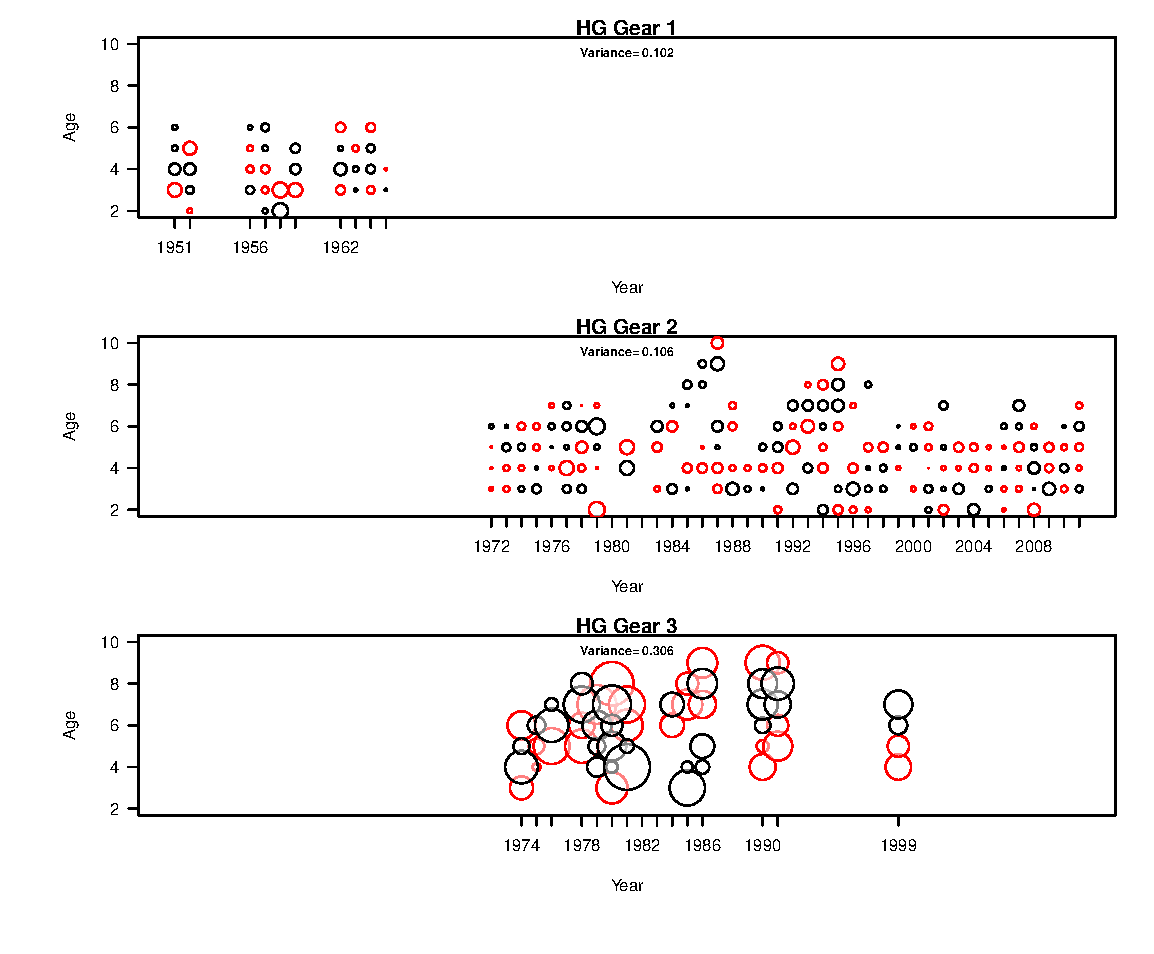
\includegraphics[width=0.9\textwidth]{../FIGS/qPriorFigs/iscam_fig_agecompsresid_HG.pdf}\\
	\caption{Residual difference between the observed and predicted proportions-at-age for HG for each of the three gear types (Gear 1 = winter seine, Gear 2 = seine-roe, Gear 3 = gill net).  The area of each circle is proportional to the residua, black is positive, and red is negative.  The corresponding MLE estimates of the residual variance is displayed in each panel.}\label{PartII:Results:figAgeCompHG}
\end{sidewaysfigure}

For the PRD region, the fits to the age-composition data are slightly poorer, with MLE estimates of the variance ranging from 0.215 to 0.358 for the seine-roe and gill net fleets (Fig. \ref{PartII:Results:figAgeCompPRD}). There is no remarkable pattern in the winter seine fishery, the seine-roe fishery tends to have positive residuals for age-3 and age 7+ fish, and negative residuals for ages 4-6 fish.  Similarly, the is an age-pattern in the residuals for the gill net fishery with negative residuals for age-4 and ages 9+ fish, and positive residuals for ages 5-8.  Residuals in 2011 age-composition data are much larger  than all other years.

\begin{sidewaysfigure}[!tbp]
	% Requires \usepackage{graphicx}
	\centering
	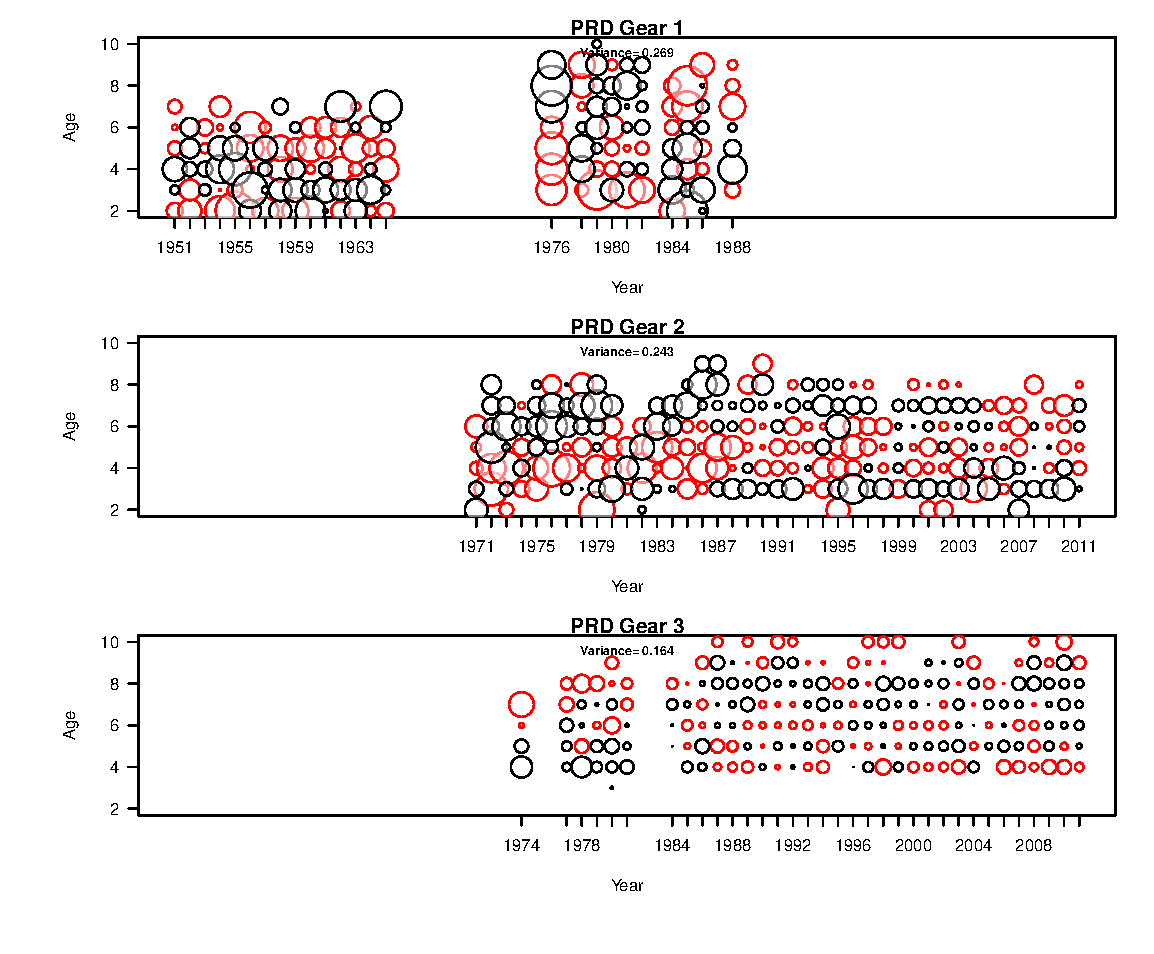
\includegraphics[width=0.9\textwidth]{../FIGS/qPriorFigs/iscam_fig_agecompsresid_PRD.pdf}\\
	\caption{Residual difference between the observed and predicted proportions-at-age for PRD for each of the three gear types (Gear 1 = winter seine, Gear 2 = seine-roe, Gear 3 = gill net).  The area of each circle is proportional to the residua, black is positive, and red is negative.  The corresponding MLE estimates of the residual variance is displayed in each panel.}\label{PartII:Results:figAgeCompPRD}
\end{sidewaysfigure}


For the Central Coast (CC) region, there is also good correspondence between the observed and predicted age-composition data, with MLE estimates of the variance ranging from 0.128 to 0.203 (Fig. \ref{PartII:Results:figAgeCompCC}).  There is no striking temporal pattern in the residuals for any of the fishing fleets.  There is a tendency to overestimate the porportion-at-age 4 and 5 in the seine-roe fishery.


\begin{sidewaysfigure}[!tbp]
	% Requires \usepackage{graphicx}
	\centering
	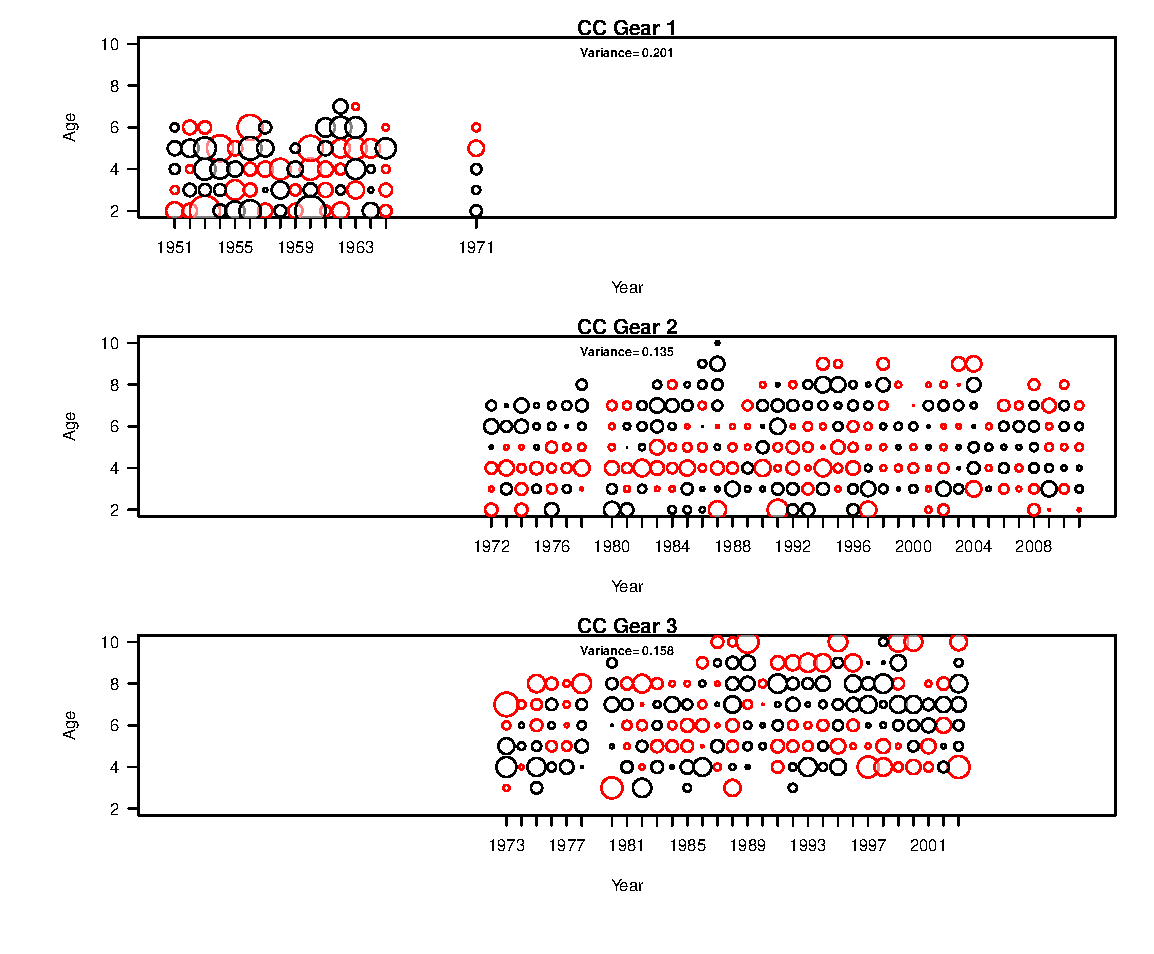
\includegraphics[width=0.9\textwidth]{../FIGS/qPriorFigs/iscam_fig_agecompsresid_CC.pdf}\\
	\caption{Residual difference between the observed and predicted proportions-at-age for CC for each of the three gear types (Gear 1 = winter seine, Gear 2 = seine-roe, Gear 3 = gill net).  The area of each circle is proportional to the residua, black is positive, and red is negative.  The corresponding MLE estimates of the residual variance is displayed in each panel.}\label{PartII:Results:figAgeCompCC}
\end{sidewaysfigure}

For the Strait of Georgia, there is also very good correspondence between the observed and predicated age-composition data for all three gears (Fig \ref{PartII:Results:figAgeCompSOG}).  The MLE estimates of the variance range from 0.088 to 0.021 for the seine-roe and gill net fleets, respectively.  In the gill net fleet  there has been a tendency to under-estimate the proportions-at-age 4-6 between the 1970s and mid 1990s and more recently to over-estimate the proportions-at-age 6-8.  Recall that selectivity for the gill net fishery is a function of the empirical weight-at-age data, which has been trending to small fish in recent years.


\begin{sidewaysfigure}[!tbp]
	% Requires \usepackage{graphicx}
	\centering
	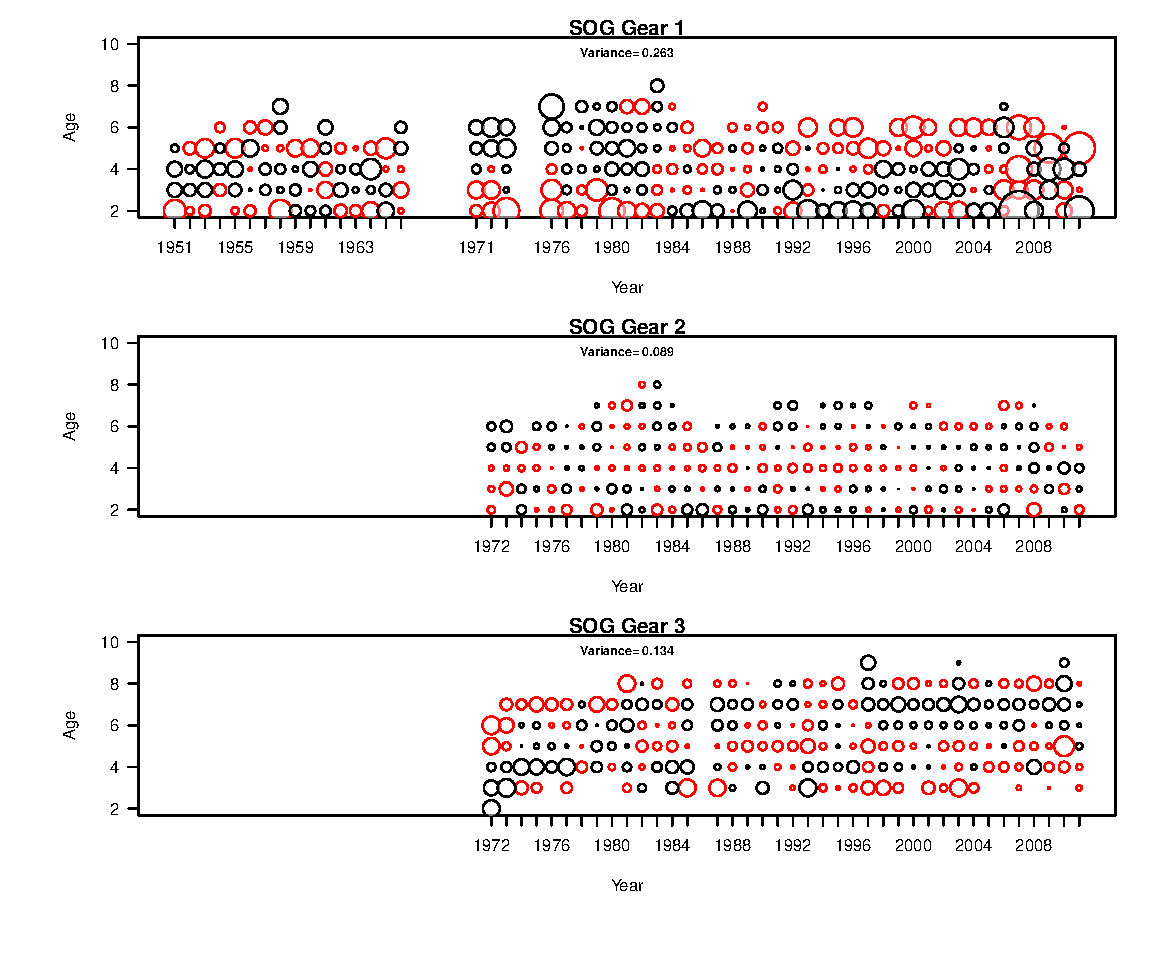
\includegraphics[width=0.9\textwidth]{../FIGS/qPriorFigs/iscam_fig_agecompsresid_SOG.pdf}\\
	\caption{Residual difference between the observed and predicted proportions-at-age for SOG for each of the three gear types (Gear 1 = winter seine, Gear 2 = seine-roe, Gear 3 = gill net).  The area of each circle is proportional to the residua, black is positive, and red is negative.  The corresponding MLE estimates of the residual variance is displayed in each panel.}\label{PartII:Results:figAgeCompSOG}
\end{sidewaysfigure}

In the case of WCVI, there is good correspondence between the observed and predicted age composition data for the seine fisheries and less so for the gill net fishery (Fig \ref{PartII:Results:figAgeCompWCVI}).  The MLE estimates of the variance range fro 0.088 to 0.314 for the seine-roe and gill net fisheries, respectively.  Residual patterns in the seine fisheries are unremarkable, perhaps an age-pattern in the seine roe fishery.  There is a tendency to under-estimate the proportions-at-age in the gill net fishery for ages 5-7.   The size of the residuals are fairly homogenous over time for all gears.


\begin{sidewaysfigure}[!tbp]
	% Requires \usepackage{graphicx}
	\centering
	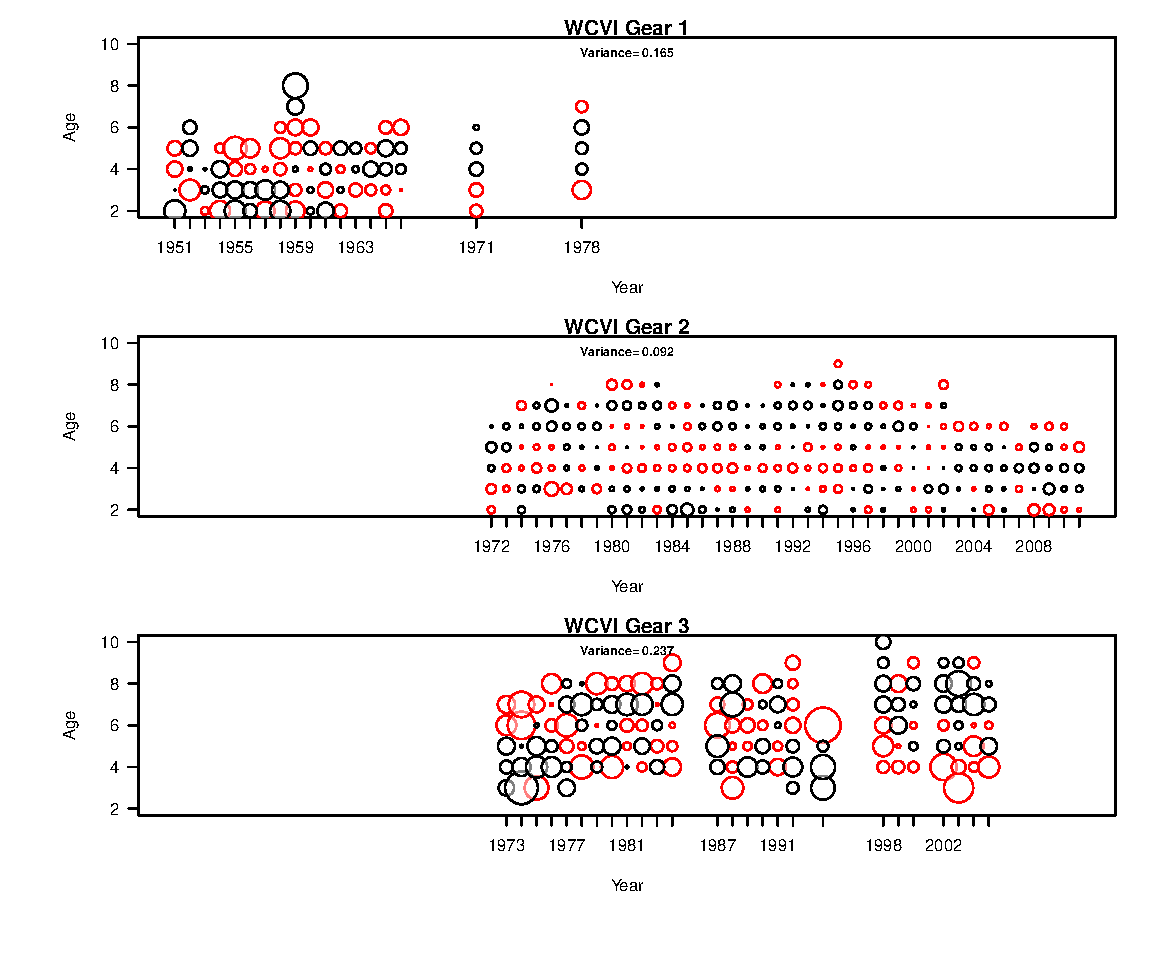
\includegraphics[width=0.9\textwidth]{../FIGS/qPriorFigs/iscam_fig_agecompsresid_WCVI.pdf}\\
	\caption{Residual difference between the observed and predicted proportions-at-age for WCVI for each of the three gear types (Gear 1 = winter seine, Gear 2 = seine-roe, Gear 3 = gill net).  The area of each circle is proportional to the residua, black is positive, and red is negative.  The corresponding MLE estimates of the residual variance is displayed in each panel.}\label{PartII:Results:figAgeCompWCVI}
\end{sidewaysfigure}


\subsection{Marginal posterior distributions}

\subsection{Forecast and catch advice based on the joint posterior distribtution}
 The catch advice in Tables \ref{TableCatchAdvice} and \ref{TableCatchAdviceqFix} is based on the old cuttoffs.


% latex.default(xTable, file = fn, rowname = NULL, longtable = FALSE,      landscape = FALSE, cgroup = cgrp, n.cgroup = ncgrp, caption = cap,      label = "TableCatchAdvice", na.blank = TRUE, vbar = FALSE,      size = "small") 
%
\begin{table}[!tbp]
 \small
 \caption{Estimated spawning stock biomass,  age-4+ biomass and pre-fishery biomass for poor average and good recruitment,  cutoffs, and available harvest under the assumption that q=1 for the contemporary spawn survey data.\label{TableCatchAdviceqFix}} 
 \begin{center}
 \begin{tabular}{lllclllclclll}\hline\hline
\multicolumn{3}{c}{\bfseries }&
\multicolumn{1}{c}{\bfseries }&
\multicolumn{3}{c}{\bfseries Pre-fishery forecast biomass}&
\multicolumn{1}{c}{\bfseries }&
\multicolumn{1}{c}{\bfseries }&
\multicolumn{1}{c}{\bfseries }&
\multicolumn{3}{c}{\bfseries Available harvest}
\tabularnewline \cline{1-13}
\multicolumn{1}{c}{Stock}&\multicolumn{1}{c}{SSB}&\multicolumn{1}{c}{4+ Biomass}&\multicolumn{1}{c}{}&\multicolumn{1}{c}{Poor}&\multicolumn{1}{c}{Average}&\multicolumn{1}{c}{Good}&\multicolumn{1}{c}{}&\multicolumn{1}{c}{Cutoff}&\multicolumn{1}{c}{}&\multicolumn{1}{c}{Poor}&\multicolumn{1}{c}{Average}&\multicolumn{1}{c}{Good}\tabularnewline
\hline
HG& 7,147& 2,736&& 4,259& 6,662&12,776&&10,700&&     0&     0& 2,076\tabularnewline
PRD&29,071& 8,427&&10,486&12,649&20,016&&12,100&&     0&   549& 4,003\tabularnewline
CC& 8,427& 4,308&& 6,720& 9,264&15,438&&17,600&&     0&     0&     0\tabularnewline
SOG&51,500&21,640&&31,921&40,236&52,616&&21,200&& 6,384& 8,047&10,523\tabularnewline
WCVI& 6,948& 3,645&& 7,404&11,373&18,438&&18,800&&     0&     0&     0\tabularnewline
\hline
\end{tabular}

\end{center}

\end{table}



% latex.default(xTable, file = fn, rowname = NULL, longtable = FALSE,      landscape = FALSE, cgroup = cgrp, n.cgroup = ncgrp, caption = cap,      label = "TableCatchAdvice", na.blank = TRUE, vbar = FALSE,      size = "small") 
%
\begin{table}[!tbp]
 \small
 \caption{Estimated spawning stock biomass,  age-4+ biomass and pre-fishery biomass for poor average and good recruitment,  cutoffs, and available harvest based on a normal prior ($\mu=0,\sigma=0.274$) for $q$ in both surveys.\label{TableCatchAdvice}} 
 \begin{center}
 \begin{tabular}{lllclllclclll}\hline\hline
\multicolumn{3}{c}{\bfseries }&
\multicolumn{1}{c}{\bfseries }&
\multicolumn{3}{c}{\bfseries Pre-fishery forecast biomass}&
\multicolumn{1}{c}{\bfseries }&
\multicolumn{1}{c}{\bfseries }&
\multicolumn{1}{c}{\bfseries }&
\multicolumn{3}{c}{\bfseries Available harvest}
\tabularnewline \cline{1-13}
\multicolumn{1}{c}{Stock}&\multicolumn{1}{c}{SSB}&\multicolumn{1}{c}{4+ Biomass}&\multicolumn{1}{c}{}&\multicolumn{1}{c}{Poor}&\multicolumn{1}{c}{Average}&\multicolumn{1}{c}{Good}&\multicolumn{1}{c}{}&\multicolumn{1}{c}{Cutoff}&\multicolumn{1}{c}{}&\multicolumn{1}{c}{Poor}&\multicolumn{1}{c}{Average}&\multicolumn{1}{c}{Good}\tabularnewline
\hline
HG&11,294& 4,937&& 6,706& 9,291&15,620&&10,700&&     0&     0& 3,124\tabularnewline
PRD&15,212& 4,323&& 5,613& 7,033&12,618&&12,100&&     0&     0&   518\tabularnewline
CC& 8,055& 4,287&& 6,428& 8,751&14,477&&17,600&&     0&     0&     0\tabularnewline
SOG&57,330&23,850&&34,828&43,739&57,119&&21,200&& 6,966& 8,748&11,424\tabularnewline
WCVI& 8,247& 4,453&& 8,729&12,857&20,180&&18,800&&     0&     0& 1,380\tabularnewline
\hline
\end{tabular}

\end{center}

\end{table}



% latex.default(xTable, file = fn, rowname = NULL, longtable = FALSE,      landscape = FALSE, cgroup = cgrp, n.cgroup = ncgrp, caption = cap,      label = "TableCatchAdvice", na.blank = TRUE, vbar = FALSE,      size = "small") 
%
\begin{table}[!tbp]
 \small
 \caption{Estimated spawning stock biomass,  age-4+ biomass and pre-fishery
			biomass for poor average and good recruitment,  cutoffs,  and 
			available harvest.\label{TableCatchAdvice}} 
 \begin{center}
 \begin{tabular}{lllclllclclll}\hline\hline
\multicolumn{3}{c}{\bfseries }&
\multicolumn{1}{c}{\bfseries }&
\multicolumn{3}{c}{\bfseries Pre-fishery forecast biomass}&
\multicolumn{1}{c}{\bfseries }&
\multicolumn{1}{c}{\bfseries }&
\multicolumn{1}{c}{\bfseries }&
\multicolumn{3}{c}{\bfseries Available harvest}
\tabularnewline \cline{1-13}
\multicolumn{1}{c}{Stock}&\multicolumn{1}{c}{SSB}&\multicolumn{1}{c}{4+ Biomass}&\multicolumn{1}{c}{}&\multicolumn{1}{c}{Poor}&\multicolumn{1}{c}{Average}&\multicolumn{1}{c}{Good}&\multicolumn{1}{c}{}&\multicolumn{1}{c}{Cutoff}&\multicolumn{1}{c}{}&\multicolumn{1}{c}{Poor}&\multicolumn{1}{c}{Average}&\multicolumn{1}{c}{Good}\tabularnewline
\hline
HG&11,294& 4,937&& 6,706& 9,291&15,620&&10,700&&     0&     0& 3,124\tabularnewline
PRD&15,068& 4,339&& 5,645& 7,015&12,699&&12,100&&     0&     0&   599\tabularnewline
CC& 8,047& 4,265&& 6,347& 8,658&14,429&&17,600&&     0&     0&     0\tabularnewline
SOG&56,358&23,195&&33,549&42,332&55,102&&21,200&& 6,710& 8,466&11,020\tabularnewline
WCVI& 7,889& 4,251&& 8,387&12,396&19,542&&18,800&&     0&     0&   742\tabularnewline
\hline
\end{tabular}

\end{center}

\end{table}





%Decision table
Notes from June Meeting:\\
Were not completely comfortable with the q estimates, but we believe the approach used to develop the informative prior for q is better than the ad hoc q=1 assumption.  Assuming $q=1$ is more conservative as there is a tendency for $q<1$ when freely estimated with an informative prior.
